%	% ****** Start of file MolecularSpinFlipLoss.tex ******
%
%
%

\documentclass[%
 reprint,
%superscriptaddress,
%groupedaddress,
%unsortedaddress,
%runinaddress,
%frontmatterverbose, 
%preprint,
%showpacs,preprintnumbers,
%nofootinbib,
%nobibnotes,
%bibnotes,
 amsmath,amssymb,
 aps,
prl,
%pra,
%prb,
%rmp,
%prstab,
%prstper,
%floatfix,
]{revtex4-1}

\usepackage{graphicx}% Include figure files
\usepackage{dcolumn}% Align table columns on decimal point
\usepackage{bm}% bold math
\usepackage[hidelinks]{hyperref}% add hypertext capabilities
%\usepackage[mathlines]{lineno}% Enable numbering of text and display math
%\linenumbers\relax % Commence numbering lines
\usepackage{textcomp}

\usepackage{color}
\newcommand{\red}[1]{{\color{black} #1}}

%\usepackage[showframe,%Uncomment any one of the following lines to test 
%%scale=0.7, marginratio={1:1, 2:3}, ignoreall,% default settings
%%text={7in,10in},centering,
%%margin=1.5in,
%%total={6.5in,8.75in}, top=1.2in, left=0.9in, includefoot,
%%height=10in,a5paper,hmargin={3cm,0.8in},
%]{geometry}


\newcommand{\bcl}{{$B_\text{coil}$}}
\newcommand{\epb}{{$\vec{E}\,{\perp}\,\vec{B}$}}
\newcommand{\epbm}{{\vec{E}\,{\perp}\,\vec{B}}}
\newcommand{\cmnt}[1]{\ignorespaces}



\begin{document}

%\preprint{APS/123-QED}

\title{Implications for Earlier Results}%

%\author{David Reens}
%\thanks{Contributed equally. Email dave.reens@colorado.edu or hao.wu@colorado.edu.}

%\author{Hao Wu}
%\thanks{Contributed equally. Email dave.reens@colorado.edu or hao.wu@colorado.edu.}

%\author{Tim Langen}%
%\altaffiliation{Present Address: 5. Physikalisches Institut and Center for Integrated Quantum Science and Technology (IQST), Universit\"at Stuttgart, Pfaffenwaldring 57, 70569 Stuttgart, Germany}

%\author{Jun Ye}
%\affiliation{JILA, National Institute of Standards and Technology and the University of Colorado and\\ Department of Physics, University of Colorado, Boulder, Colorado 80309-0440, USA}


%\date{\today}

\maketitle


%%%%%%%%%%%%%%%%%%%%%%%%%%%%%%%%%
%     COPY FROM WORD DOC
%%%%%%%%%%%%%%%%%%%%%%%%%%%%%%%%%

The present study on the role of mixed fields for spin-flip loss introduces important modifications to previously published work, especially references~\cite{Stuhl2012evap,Stuhl2013} which study collisional processes in OH molecules in a spin-flip prone geometry. 
Both of these results are considerably weakened by our present results, but perhaps not entirely overturned. 
In what follows we provide the interested reader with our current best understanding of the situation.

We begin with~\cite{Stuhl2013} on E-field induced inelastic collisions. 
During the course of analysis of the data for this work, the authors uncovered and investigated the same single particle spin-flip loss enhancement process we discuss in the present work, and an attempt was made at deconvolution. 
An appendix of~\cite{Stuhl2013} explains this well. 
Since then, in addition to further exploring the generality of the effect and conclusively demonstrating and overcoming it in a dedicated system as described in the main text, we have made an important correction to the mathematics in the appendix of~\cite{Stuhl2013}.

We make the same simplifying assumptions: loss only occurs in the \epb{} plane, only the velocity orthogonal to this plane matters ($v_z$ in the main text and $v_\theta$ in~\cite{Stuhl2013} are mathematically equivalent where \epb{}), and a thermalized Maxwell-Boltzmann distribution.
The divergence occurs with regard to the integral calculation for the loss rate.
In~\cite{Stuhl2013} integration over the entire spatial distribution is performed, weighted by the frequency of crossing of the center plane:
\begin{equation}
\Gamma_\text{LZ}=\int_0^\infty4\pi r^2n(r)dr\int_0^\infty n(v_\theta)dv_\theta \frac{v_\theta}{\pi r} P_\text{hop}(r,v_\theta)
\end{equation}
Here $n(r)$ is the radial distribution function, constrained to satisfy $\int_0^\infty 4\pi r^2n(r)=1$, and of the form $n(r)\propto e^{-\mu_BB`r/kT}$. 
Likewise $n(v_\theta)$ is the usual normalized Maxwellian velocity distribution. 
Implicit in this integration is the approximation that molecules at a given radius $r$ at a given instant will cross the center plane with a frequency of $v_\theta/\pi r$.
Though not a bad place to start, this approximation is rather rough given that molecules are certainly not following circular orbits of constant $v_\theta$ but are in general following some unusual linear trap motion.
Moreover, the strong-weak asymmetry of the trap is not treated.
Instead, we perform an integration of flux through the loss plane directly:
\begin{equation}
\Gamma_\text{LZ}=\int_0^\infty2\pi r n(r)dr\int_0^\infty n(v_z)dv_z v_z P_\text{hop}(r,v_z)
\end{equation}
Here the distributions are as before, but the radial distribution is integrated over the central plane, hence the $2\pi r$ Jacobean, and the hopping probability integrand is multiplied by the velocity $v_z$ since this sets the flux through the plane.
Under the same simplifying assumptions, this flux integral gives the desired loss rate without any approximations about molecule orbits or plane-crossing frequency.
Although the two integrals differ significantly in their conception, mathematically the changes to the integrand and the Jacobeans cancel one another out and the difference reduces to precisely an overall scaling factor of $\pi$. 

The influence of this on the deconvolution procedure is subtle, and requires getting a bit deeper into the extraction of two-body loss rates from the data. 
Essentially one plus two body fits were performed to various decay trap curves, with the one body component fixed to the value expected due to vacuum scattering and spin-flip loss.
The problem is that with the stronger spin-flip loss, it seems no longer appropriate to assume this loss will be present in the data as a pure one-body decay.
Rather, if the loss rate is faster than any thermalization rate, molecules whose trajectory naturally takes them through the loss region will be lost within a few oscillations, and thereafter the loss reduces to some lower value.
This means that the spin-flip loss can actually masquerade as a two-body population curve, since it can lead to a loss rate that decreases over time.
When we perform simulations to investigate this, we obtain curves such as shown in fig.~\ref{fig:eil}.
The curves certainly do a decent job matching the magnitude of the loss induced by the electric field, and they do predict a loss rate that turns off over time.
Nonetheless they don't really match the data regarding the initial slope of the loss.
This could be related to details of the escape of the molecules after spin-flips, which in general involve several intermediate and partially trapped sub-states of OH.

\begin{figure}[tb]
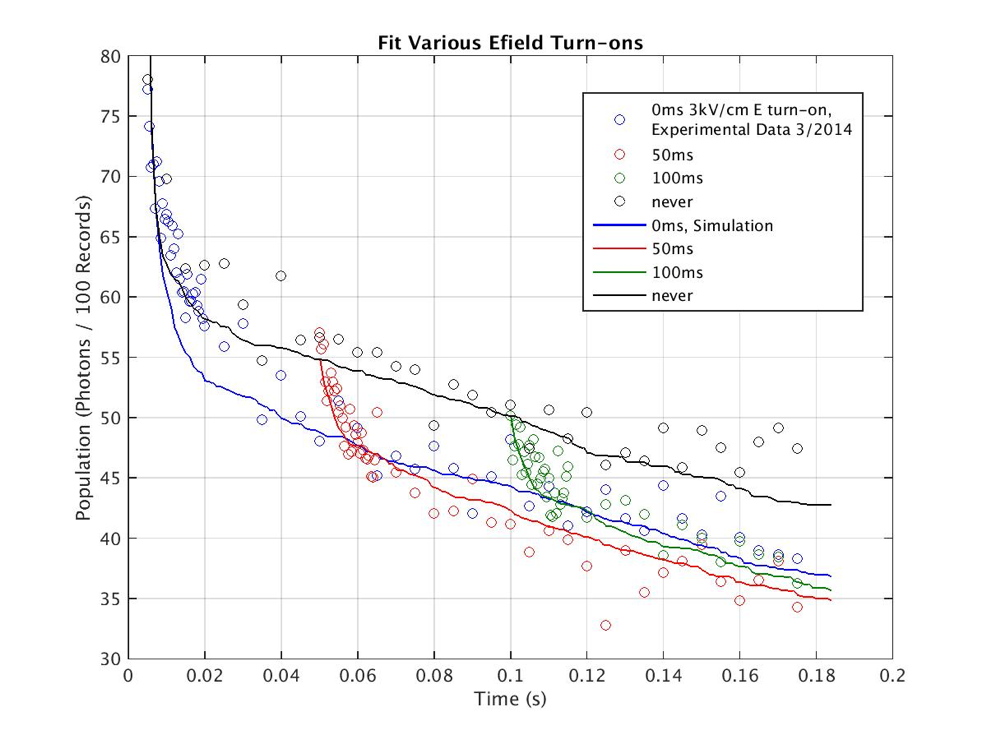
\includegraphics[width=\linewidth]{SuppFigs/EIL.png}%
\caption{
Experimental E-filed induced loss data with an attempted overlap to spin-flip loss simulations.
}
\label{fig:eil}
\end{figure}

If we perform a two body fitting procedure like the one used in~\cite{Stuhl2013} to the data obtained in this single particle simulation, we can obtain the curve shown in~\ref{fig:beta}. 
This suggests that the effect attributed to two-body collisions could be explained entirely by spin-flip losses.
Nonetheless, there are many challenges in the quantitative application of simulations such as these, especially when thermalization may not be efficient enough to smooth out the uncertainty in the initial distribution loaded after Stark deceleration.
We think the best path forward is to perform future collisional studies with the single-particle effect removed, as described in the main text.

\begin{figure}[tb]
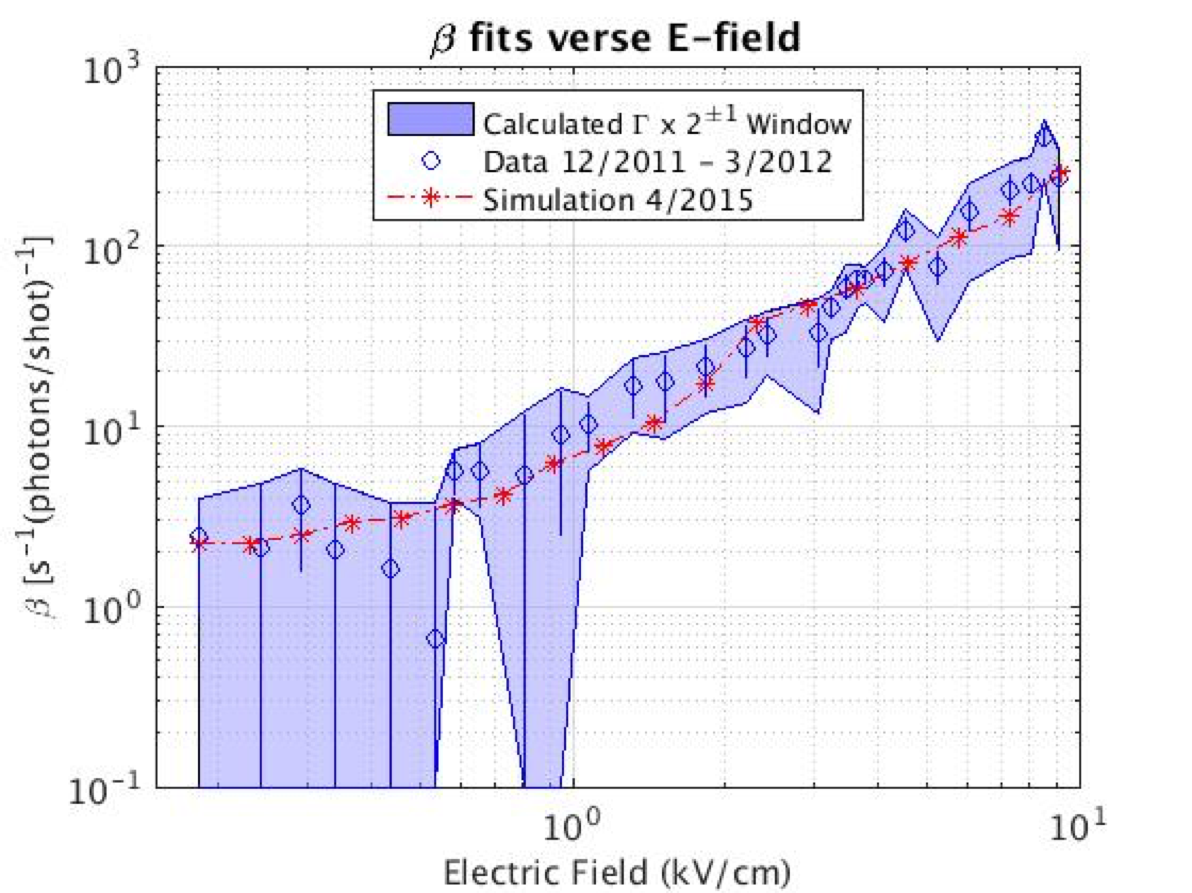
\includegraphics[width=\linewidth]{SuppFigs/Beta.png}%
\caption{
Two body fits from~\cite{Stuhl2013} with overlapped spin flip loss single particle simulation in red stars.
}
\label{fig:beta}
\end{figure}

With regard to~\cite{Stuhl2012evap}, the present study is only one of a number of important modifications to our understanding that have come up in the past few years. The first is related to the approximate Hamiltonian used for interpretation of microwave spectroscopies. As discussed in~\cite{Maeda2015}, centrifugal perturbations result in a $15\%$ correction to the inferred magnetic field at a particular microwave frequency. This would only shift the fitted temperatures slightly colder, except that it also changes the location of avoided crossings, and renders the assumption of a Boltzmann suppression factor related to these crossings untenable. The data show a sudden suppression below $480\text{ G}$, but the crossing is actually located closer to $400\text{ G}$. Without this, the fits used to calculate temperature when the population ought to be significantly built-up at lower magnetic fields are no longer trustworthy. 

In fact, the unreliability of the deeper cutting spectra in~\cite{Stuhl2012evap} ( all but the shallowest, panel (c) of figure 3) is the same conclusion implied by the present study of spin-flip losses, which show that at low temperatures the spin-flip loss caused by the electric field used during evaporation are too large. It is still possible to ignore the fits, and use the normalized spectra to look for any enhancements in density at fields below the evaporation endpoint. Normalization does become harder to do properly without a fitting function, as integrated curve area necessarily conglomerates point uncertainty, but nonetheless our routines consistently demonstrate some enhancement, see fig.~\ref{fig:normenhance}.

\begin{figure}[tb]
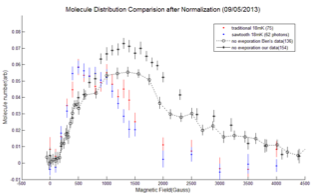
\includegraphics[width=\linewidth]{SuppFigs/NormEnhance.png}%
\caption{
Two body fits from~\cite{Stuhl2013} with overlapped spin flip loss single particle simulation in red stars.
}
\label{fig:normenhance}
\end{figure}

We have also developed a few more sensitive tools to look for collisional or evaporative effects. One is to compare the populations under two related conditions- the first a normal evaporation sequence and the second an evaporation with time-reversed microwave frequency. In other words, the cut goes backwards from deep to shallow. This comparison subjects all molecules to the same integrated microwave power, and thus the two conditions would be equivalent in a situation with only single particle effects. With evaporative effects, the normal condition ought to perform better. This is indeed what we consistently observe, at the 5\% level, see fig.~\ref{fig:normenhance}.

Another tool we have pursued is the precise calibration of our LIF system, using a careful comparison to Raman scattering of $\text{H}_2$, as described in~\cite{Bischel1986}. Our results suggest that since 2014, our molecule number has been in the $1000$ range, yielding a peak density of $10^7/\text{cm}^3$ assuming a thermal distribution, and a collision rate of not more than $0.1/\text{s}$. This value would be far too low even for a slight evaporation during a $100\text{ ms}$ experiment, but it is possible that some decline in system performance could be involved, since we have a record of decreased voltage conditioning performance in our decelerator.

A final tool is the ability to reduce our density in a tunable manner. It is crucial for such a tool to reduce density without any perturbation to the distribution of the molecules, and for this reason we have not successfully developed such a tool before. For example, reducing the initial partial pressure of water at the very beginning of our experiment would require a temperature change that would influence the initial speed of the molecules. We have settled on microwaves applied at low power during deceleration to couple strong and weak field seeking states and lead to a uniform escape probability for the molecules. This tool enables searches for collisional effects by comparing experiments performed identically except for changes in the density of OH molecules. Unfortunately it can only do so by reducing the density, when obviously collisional effects would be most evident upon increasing it.

In conclusion, the collisional results in~\cite{Stuhl2012evap,Stuhl2013} are significantly weakened by spin-flip losses and some other modifications to our understanding. The density may simply have been too low, although back-application to the 2012-13 systems used is not perfect. Nonetheless spectroscopic comparisons and evaporation subtractions still suggest a slight evaporative effect, and the development of various more sensitive tools has us poised to more unambiguously identify any future collisional effects in our next generation system described in the main text.

%includes uncited bib entries
%\nocite{*}
\bibliographystyle{apsrev4-1_no_Arxiv}
\bibliography{Supplement}

\end{document}
%
% ****** End of file MolecularMajoranaLoss.tex ******
